\chapter{Desarrollo}

\section{Map4rdf}
\subsection{Instalacion}

Se ha optado por utilizar la maquina Virtual proporcionada en la Wiki del proyecto para minimizar la posibilidad
de incompatibilidades.

\section{GeoKettle}

Desde que se publico ``A sustainable process and toolbox for geographical linked data generation and
publication: a case study with BTN100'' en 2019, GeoKettle ha dejado de estar soportado. La pagina oficial y de
documentacion ya no estan disponibles.
Un objetivo de este TFG es dar soporte GeoPackage a GeoKettle. No tiene sentido desarrollar soluciones de
``modernizacion'' sobre software abandonado.

Algunas funcionalidades de GeoKettle se integraron en PDI directamente y otras desaparecieron. 
Actualmente, el soporte GIS de Pentaho esta dentro de PDI Spoon y ademas hay algunas funcionalidades mas en
 el plugin llamado pentaho-gis-plugins\cite{gis-plugins}. Se actualizara la primera fase a:
\textbf{``replicar la funcionalidad y las transformaciones de GeoKettle + TripleGeo en la suite PDI.''}. 
Dado que se trata de replicar la funcionalidad anterior, se analizaran las tranformaciones realizadas por el OEG
en el repositorio de GitHub BTN100. Como se puede ver en la figura \ref{fig:spoon-missing-plugins}, partes del
workflow fallan. Es lo que se pretende solucionar.

\begin{figure}[H]
    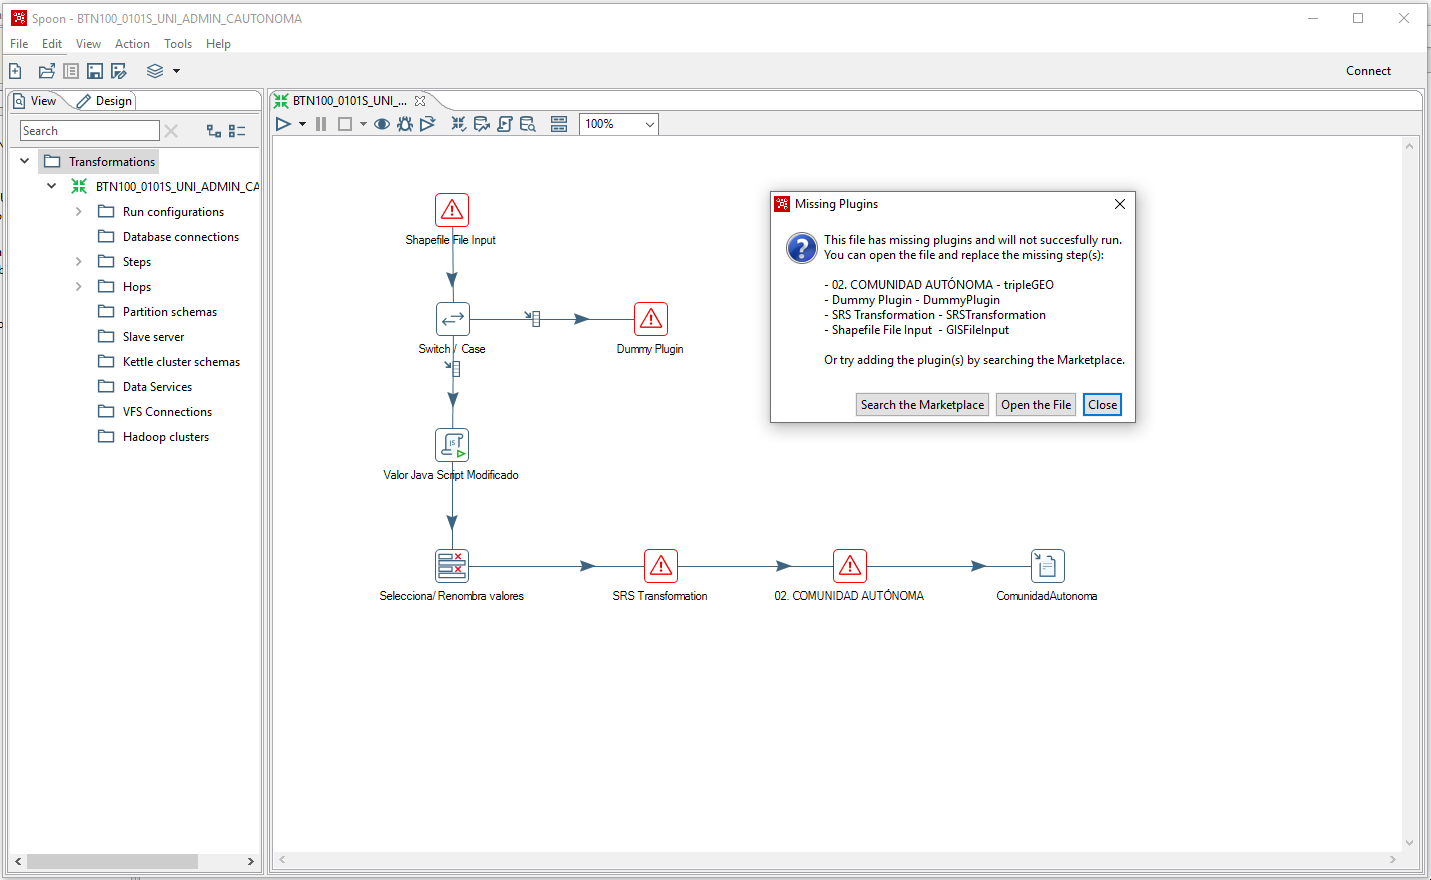
\includegraphics[width=\textwidth]{images/spoon-missing-plugins.png}
    \centering
    \caption{Workflow importado en la nueva suite}
    \label{fig:spoon-missing-plugins}
\end{figure}

\newpage
\subsection{Funcionamiento}

Para poder realizar el ``port'' de GeoKettle a Spoon, primero es necesario entender el funcionamiento y
transformaciones actuales de GeoKettle observando la entrada y salida de cada paso. Ademas esta manera se
observara mejor el flujo de datos y sera mas facil anyadir soporte a GeoPackage en el futuro. No todas las
transformaciones tienen los mismos pasos, pero son parecidas. Como ejemplo se utilizaran los datos de
BTN100\_0101S\_UNI\_ADMIN y la transformacion BTN100\_0101S\_UNI\_ADMIN\_CAUTONOMA. La transformacion contiene
los siguientes pasos:

\begin{figure}[H]
    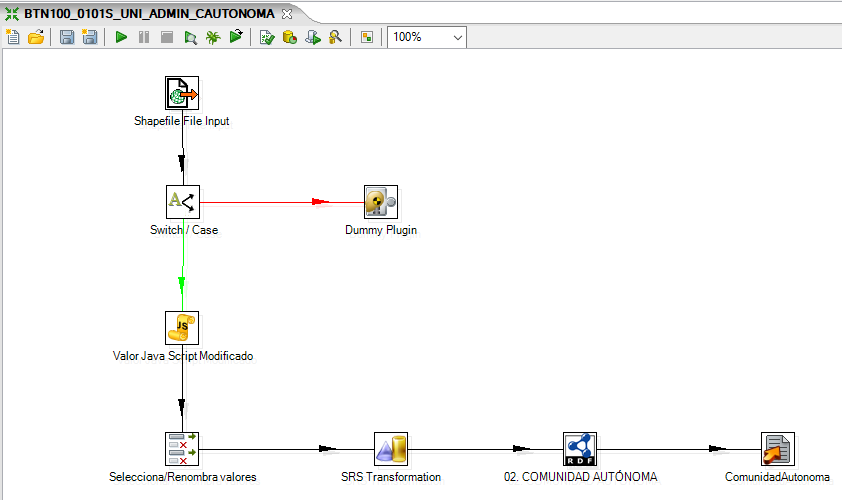
\includegraphics[width=\textwidth]{images/CCAA.png}
    \centering
    \caption{Transformacion BTN100\_0101S\_UNI\_ADMIN\_CAUTONOMA}
    \label{fig:CCAA}
\end{figure}


\begin{enumerate}
    \item Shapefile File Input
    \item Switch Case
    \item Dummy Plugin
    \item Valor Java Script Modificado
    \item Selecciona/Renombra valores
    \item SRS Transformation
    \item TripleGeo
    \item Text Output
\end{enumerate}


\subsubsection{Shapefile File Input}

Lee el fichero shapefile.
\begin{enumerate}
    \item \textit{.shp}: Geometria fig.\ref{fig:shapefile}

        \begin{figure}[H]
            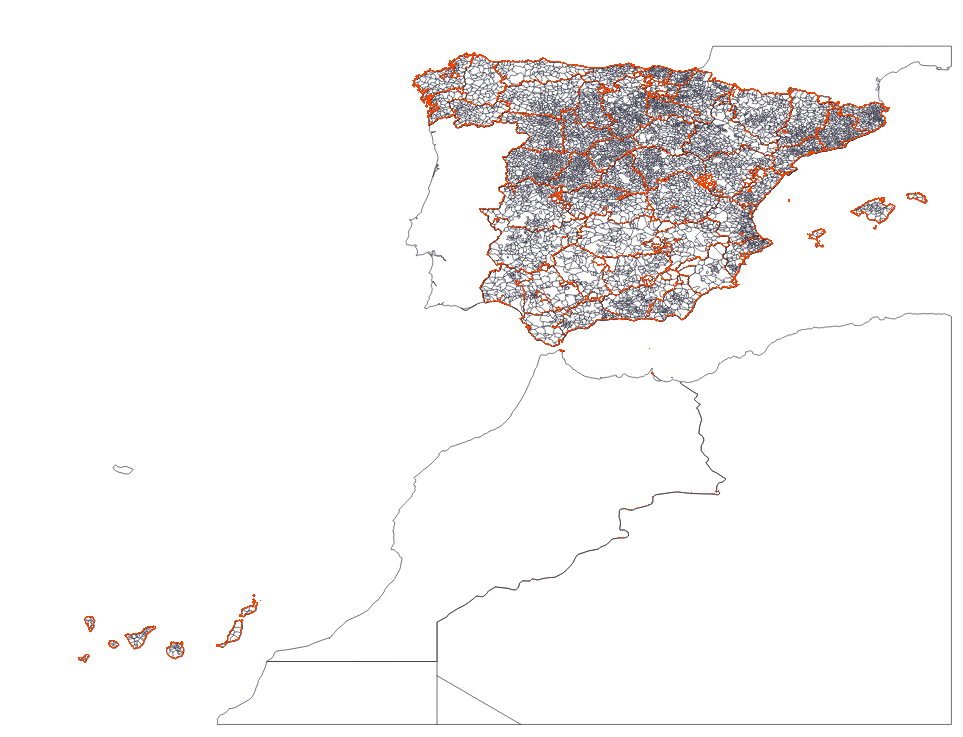
\includegraphics[width=0.7\textwidth]{images/shapefile.png}
            \centering
            \caption{Geometria contenida en el shapefile}
            \label{fig:shapefile}
        \end{figure}

    \item \textit{.dbf}: Datos asociados en columnas fig.\ref{fig:dbf}

        \begin{figure}[H]
            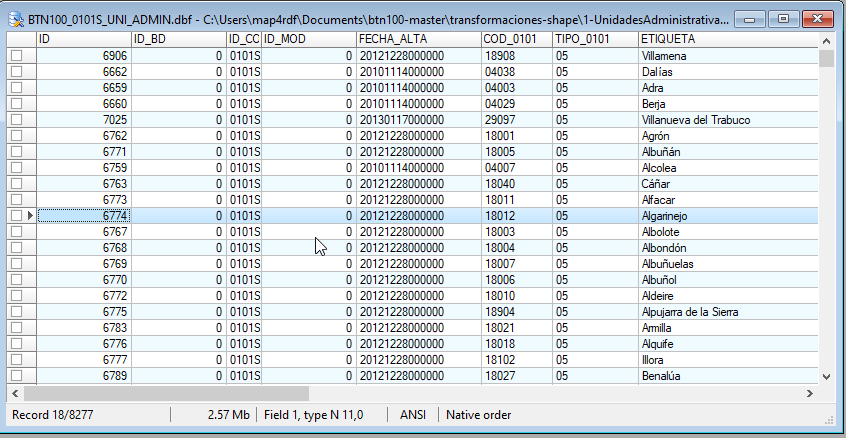
\includegraphics[width=0.7\textwidth]{images/dbf.png}
            \centering
            \caption{Datos columnares dbf asociados a la geometria}
            \label{fig:dbf}
        \end{figure}

    \item \textit{.shx}: Índice para acelerar busquedas
    \item \textit{.prj}: Sistema de coordenadas
\end{enumerate}

\subsubsection{Switch case}
El switch case se encarga de filtrar y seleccionar las comunidades autonomas, identificadas por el valor 02 del
Campo TIPO\_0101. Si son una CCAA, se envian al paso 4, e.o.c. se envian al paso 3. fig.\ref{fig:switch} y
\ref{fig:tipo02}

\begin{figure}[H]
    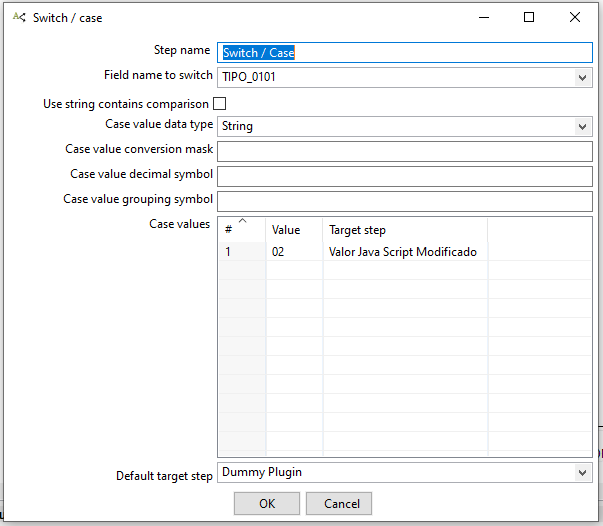
\includegraphics[width=0.7\textwidth]{images/switch.png}
    \centering
    \caption{Paso switch}
    \label{fig:switch}
\end{figure}

\begin{figure}[H]
    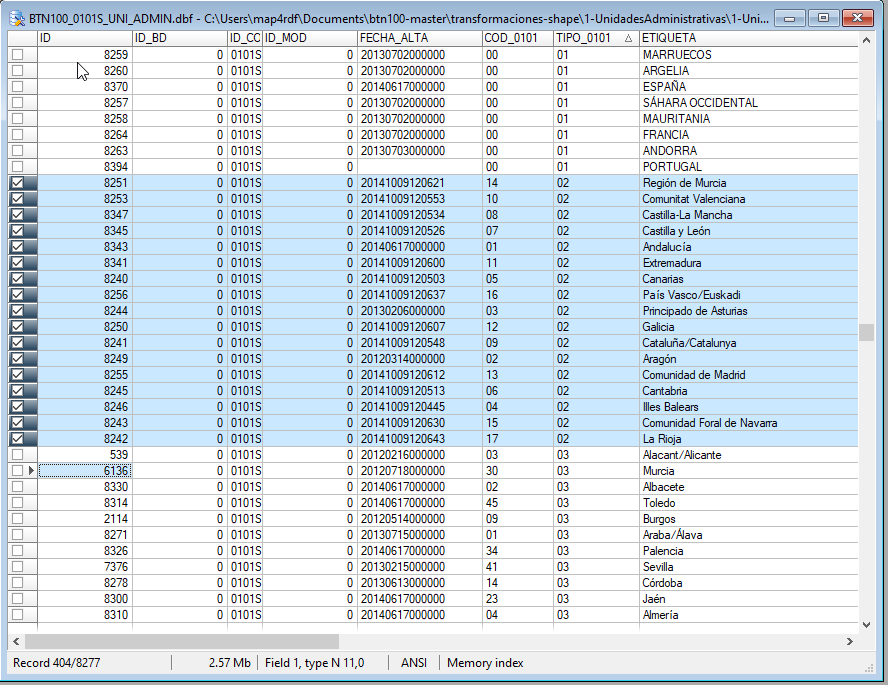
\includegraphics[width=\textwidth]{images/tipo02.png}
    \centering
    \caption{La filas correspondientes a las CCAA}
    \label{fig:tipo02}
\end{figure}

\subsubsection{Dummy Plugin}
No hace ninguna transformacion, su proposito es recoger los datos innecesarios del switch.

\subsubsection{Valor Java Script Modificado}
El script cambia el formato de la fecha para facilitar la lectura: de YYYYMMDDHHMMSS a YYYY-MM-DD. Tambien
crea un nuevo campo llamado identificador a partir del campo etiqueta, cambiando espacios por barras bajas, mayusculas
por minusculas, quitando tildes y signos de puntuacion. fig.\ref{fig:script} y \ref{fig:fecha}

\begin{figure}[H]
    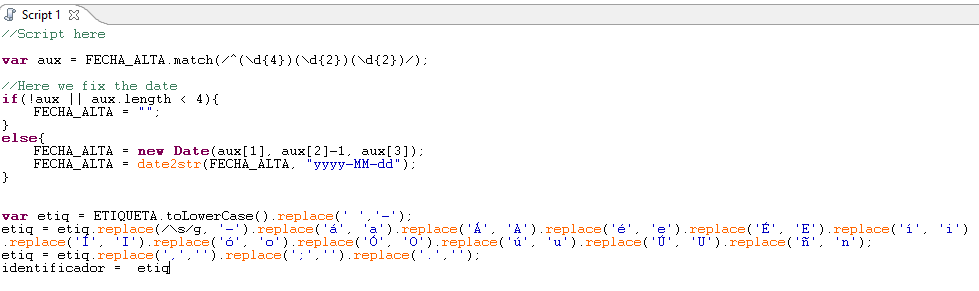
\includegraphics[width=\textwidth]{images/script.png}
    \centering
    \caption{Script Javascript}
    \label{fig:script}
\end{figure}

\begin{figure}[H]
    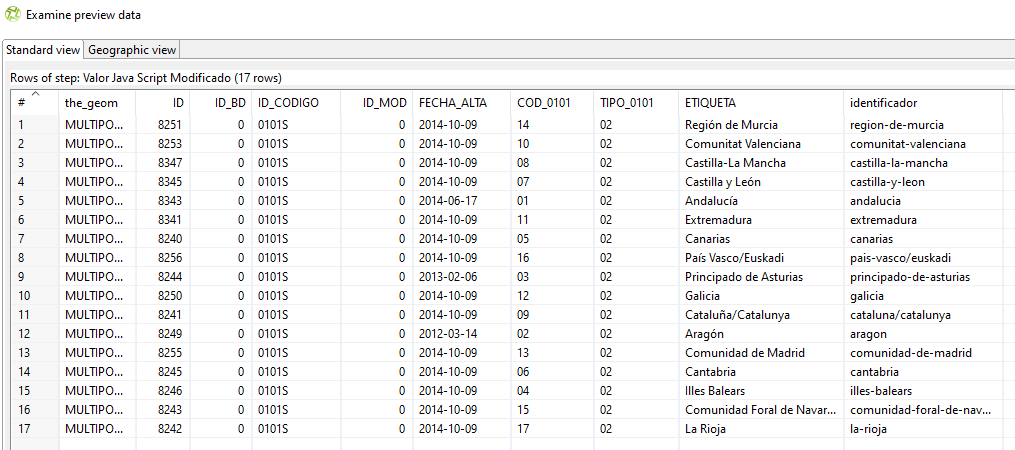
\includegraphics[width=\textwidth]{images/fecha.png}
    \centering
    \caption{Resultado del cambio de formato de fecha}
    \label{fig:fecha}
\end{figure}

\subsubsection{Selecciona/Renombra valores}
Cambia los metadatos de la columna FECHA\_ALTA para que sea reconocida como fecha. fig.\ref{fig:selecciona-renombra}

\begin{figure}[H]
    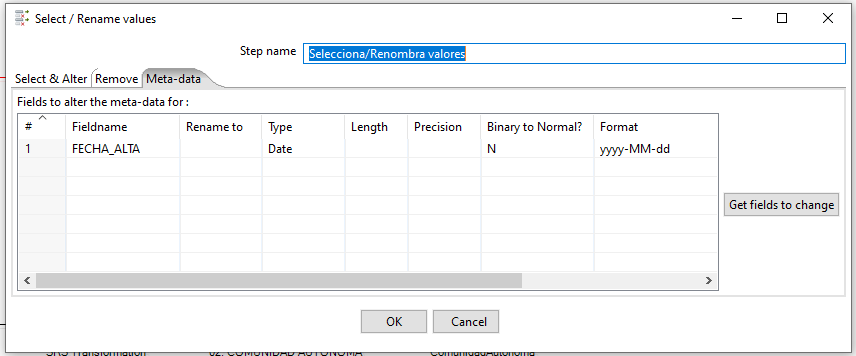
\includegraphics[width=\textwidth]{images/selecciona-renombra.png}
    \centering
    \caption{Selecciona/renombra valores}
    \label{fig:selecciona-renombra}
\end{figure}

\subsubsection{SRS Transformation}
Realiza la reproyeccion del sistema de coordenadas, en este caso de ETRS89 a WGS84. fig.\ref{fig:SRS}

\begin{figure}[H]
    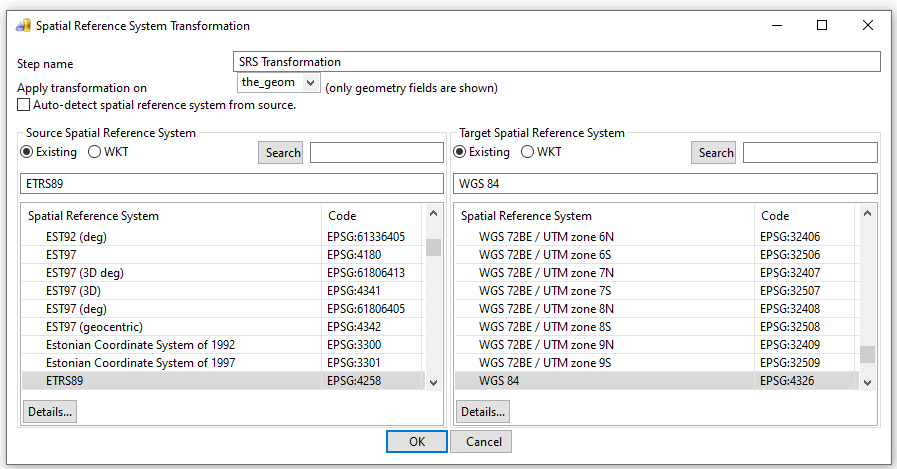
\includegraphics[width=\textwidth]{images/SRS.png}
    \centering
    \caption{Transformacion SRS}
    \label{fig:SRS}
\end{figure}

\subsubsection{TripleGeoKettle}
Transforma el shapefile del paso anterior en RDF en formato ttl. Se pueden configurar los parametros asociados a la
ontologia y decidir si se muestran ciertas columnas o no. fig.\ref{fig:tripleGeoKettle}


\begin{figure}[H]
    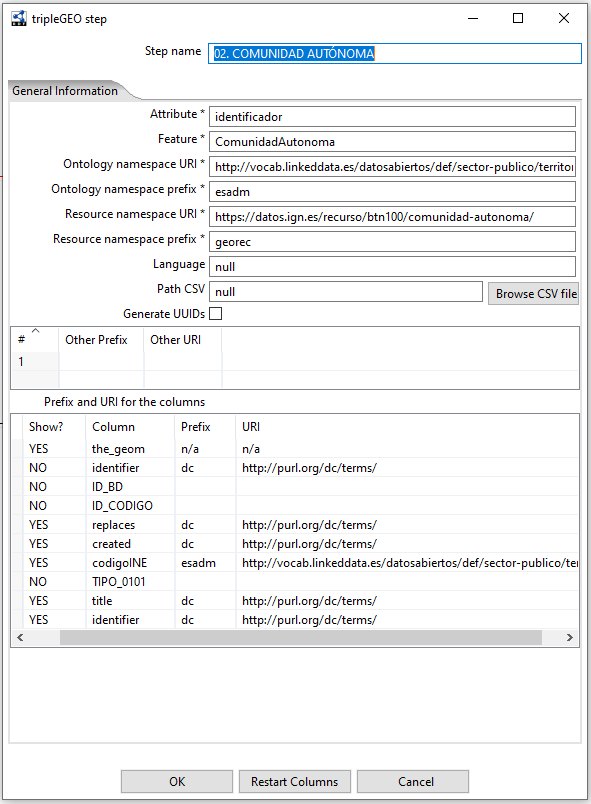
\includegraphics[width=0.9\textwidth]{images/tripleGeoKettle.png}
    \centering
    \caption{tripleGeoKettle}
    \label{fig:tripleGeoKettle}
\end{figure}

\subsubsection{Text file output}
Escribe los datos RDF en un fichero de texto con formato .ttl. fig.\ref{fig:text-file-output}
\begin{figure}[H]
    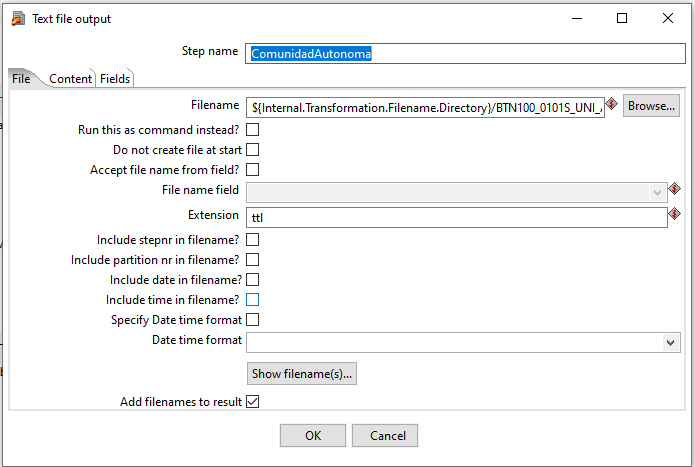
\includegraphics[width=\textwidth]{images/text-file-output.png}
    \centering
    \caption{text-file-output}
    \label{fig:text-file-output}
\end{figure}

\subsubsection{Resultado de la transformacion}
\footnotesize
\begin{verbatim}
@prefix geo:   <http://www.w3.org/2003/01/geo/wgs84_pos#> .
@prefix geosparql: <http://www.opengis.net/ont/geosparql#> .
@prefix sf:    <http://www.opengis.net/ont/sf#> .
@prefix rdf:   <http://www.w3.org/1999/02/22-rdf-syntax-ns#> .
@prefix owl:   <http://www.w3.org/2002/07/owl#> .
@prefix xsd:   <http://www.w3.org/2001/XMLSchema#> .
@prefix georec: <https://datos.ign.es/recurso/btn100/comunidad-autonoma/> .
@prefix esadm: <http://vocab.linkeddata.es/datosabiertos/def/sector-publico/territorio#> .
@prefix rdfs:  <http://www.w3.org/2000/01/rdf-schema#> .
@prefix foaf:  <http://xmlns.com/foaf/0.1/> .
@prefix dc:    <http://purl.org/dc/terms/> .

georec:comunidad-de-madrid
        a                      esadm:ComunidadAutonoma ;
        rdfs:label             "comunidad-de-madrid" ;
        dc:created             "2014-10-09"^^xsd:date ;
        dc:identifier          "comunidad-de-madrid" ;
        dc:title               "Comunidad de Madrid" ;
        esadm:codigoINE        "13"^^xsd:int ;
        geosparql:hasGeometry  <https://datos.ign.es/recurso/btn100/comunidad-autonoma/...

georec:region-de-murcia
        a                      esadm:ComunidadAutonoma ;
        rdfs:label             "region-de-murcia" ;
        dc:created             "2014-10-09"^^xsd:date ;
        dc:identifier          "region-de-murcia" ;
        dc:title               "Region de Murcia" ;
        esadm:codigoINE        "14"^^xsd:int ;
        geosparql:hasGeometry  <https://datos.ign.es/recurso/btn100/comunidad-autonoma/...

<https://datos.ign.es/recurso/btn100/comunidad-autonoma/aragon/geometry>
        a                sf:Polygon ;
        geosparql:asWKT  "POLYGON ((-1.6174492000010632 40.94373283914169, -1.62366030000...
        ...
\end{verbatim}
\normalsize


\section{Port a PDI9}

\subsection{Tests con pentaho-gis-plugins}

El 3 de Marzo el plugin anyadio soporte para el formato GeoPackage. Con el siguiente test se comprueba que los
componentes que se utilizaran para reemplazar las transformaciones antiguas funcionan correctamente.

\begin{figure}[H]
    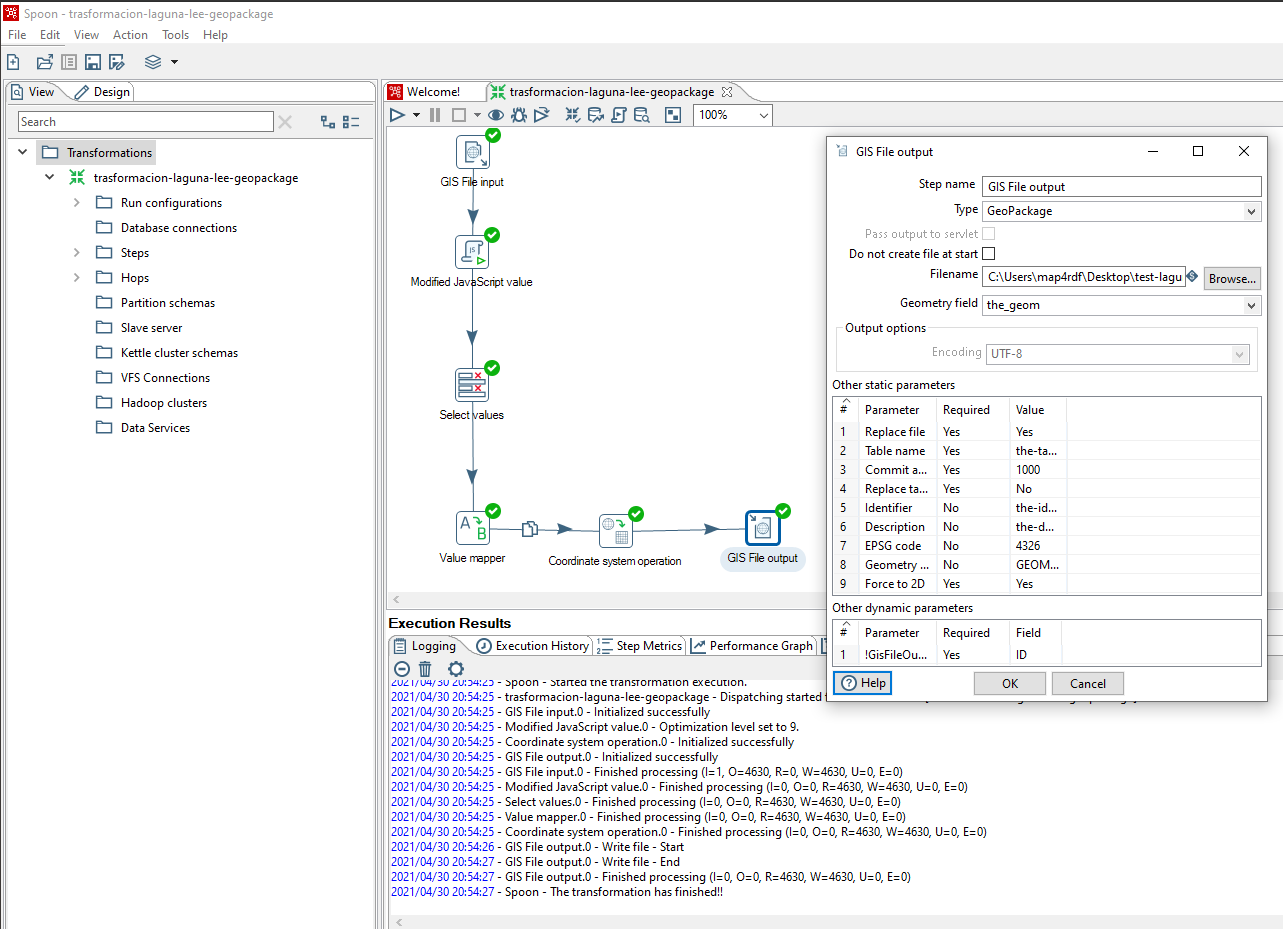
\includegraphics[width=\textwidth]{images/test-laguna-geopackage.png}
    \centering
    \caption{test-laguna-geopackage}
    \label{fig:test-laguna-geopackage}
\end{figure}

\subsection{Entorno de desarrollo}

\subsubsection{Dependencias e instalacion}

En los ultimos anyos Pentaho ha pasado de utilizar Apache Ant a utilizar Apache Maven. TripleGeoKettle tambien
utilizaba Ant, y se ha decidido utilizar Maven por las ventajas que ofrece. El proyecto TripleGeoKettle contenia
una carpeta lib en la que se encontraban los .jar con las dependencias necesarias. Ahora, las dependencias se
administran con Maven y el pom.xml. Se incluyen los repositorios de Pentaho y OSGeo y las dependencias que se
quieren incluir. Las properties funcionan a modo de ``variable'' para poder cambiar la version de pdi facilmente
en un solo lugar.


\lstinputlisting[language=XML]{code/pom-old.xml}

A continuacion se muestran los pasos para configurar el entorno de desarrollo en Arch Linux:

\begin{lstlisting}
# Instalar PDI desde AUR (los mirrors son mas rapidos que los de SourceForge)
yay -S pdi-ce
# Instalar Java 8
sudo pacman -S jdk8-openjdk
# Cambiar la version de java con
sudo archlinux-java set java-8-openjdk
# Instalar el Plugin de desarrollo
https://sourceforge.net/projects/pentaho/files/Pentaho%209.1/plugins/kettle-sdk-plugin-assembly-9.1.0.0-324.zip/download
# Instalar Maven
sudo pacman -S maven
# Descargar el settings.xml del repositorio de github en ~/.m2
https://raw.githubusercontent.com/pentaho/maven-parent-poms/master/maven-support-files/settings.xml
# Desde el directorio del plugin compilar y empaquetar el plugin
mvn clean package
# Instalarlo en PDI9 copiando el contenido del .zip generado en el directorio target
sudo cp target/tripleGeoKettle-oeg-1.jar /opt/pdi/plugins/steps/tripleGeoKettle-oeg-1/
\end{lstlisting}

\subsubsection{Pentaho sdk plugins}

Pentaho ofrece plugins\cite{pdi-sdk} muy sencillos de ejemplo que muestran como implementar un plugin. Para el port de
TripleGeoKettle se ha utilizado como referencia kettle-sdk-step-plugin que simplemente escribe Hello World. Con
el se ha probado la compilacion, el pom.xml customizado, y pruebas varias como cambiar el icono o el nombre.


\section{Proceso de porteo}

\subsection{Disenyo del plugin}



Se comienza con el sdk de Pentaho y se realizan los cambios necesarios para integrar TripleGeoKettle en el nuevo
entorno. Se muestran las imagenes del antes y despues de la estructura de carpetas. fig.\ref{fig:directorios-sdk}
y \ref{fig:directorios-TGK}

\begin{figure}[H]
    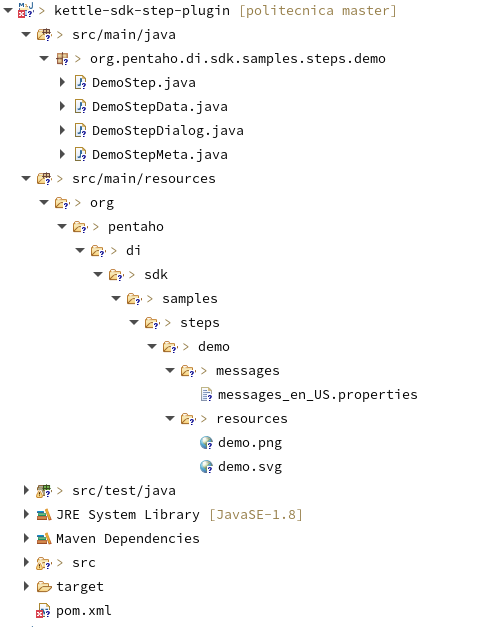
\includegraphics[width=0.7\textwidth]{images/directorios-sdk.png}
    \centering
    \caption{Estructura de carpetas del sdk}
    \label{fig:directorios-sdk}
\end{figure}

\begin{figure}[H]
    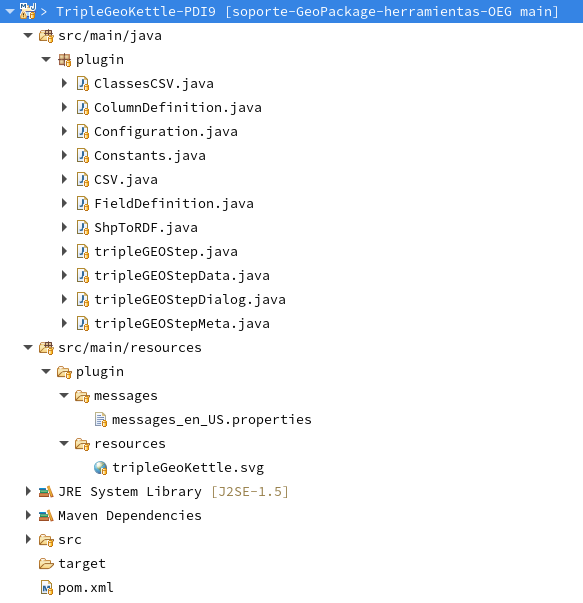
\includegraphics[width=0.7\textwidth]{images/directorios-TGK.png}
    \centering
    \caption{Estructura de carpetas de TripleGeoKettle portado}
    \label{fig:directorios-TGK}
\end{figure}

\textbf{Pasos seguidos:}

\begin{enumerate}
    \item Cambiar el nombre del paquete a ``plugin''. Es importante que el de java y el de resources tengan el
        mismo nombre para que los dialogos lean el fichero properties correctamente.

    \item Cambiar messages.properties
\begin{lstlisting}
#sdk properties
tripleGEO.FieldName.Label=Output field name
tripleGEO.CheckResult.ReceivingRows.OK=Step is receiving input from other steps.
tripleGEO.CheckResult.ReceivingRows.ERROR=No input received from other steps!

tripleGEOStep.Name=TripleGeoKettle
tripleGEOStep.TooltipDesc=An ETL Tool for Transforming Geospatial Data into RDF under the GeoSPARQL standard.
tripleGEOStep.DocumentationURL=https://github.com/oeg-upm/geo.linkeddata.es-TripleGeoKettle/wiki
tripleGEOStep.CasesURL=https://github.com/oeg-upm/geo.linkeddata.es-TripleGeoKettle/issues
tripleGEOStep.ForumURL=https://github.com/oeg-upm/geo.linkeddata.es-TripleGeoKettle/issues
tripleGEOStep.Linenr=Linenr {0}
tripleGEOStep.Error.NoOutputField=Could not find Output Field in row

# tripleGeoKettle custom properties
tripleGEOStepDialog.Shell.Title=tripleGEO step
tripleGEOStepDialog.Tab.MainTab=General Information
tripleGEOStepDialog.AttributeName.Label=Attribute *
tripleGEOStepDialog.Feature.Label=Feature *
tripleGEOStepDialog.OntologyNS.Label=Ontology namespace URI *
tripleGEOStepDialog.OntologyNSPrefix.Label=Ontology namespace prefix *
tripleGEOStepDialog.ResourceNS.Label=Resource namespace URI *
tripleGEOStepDialog.ResourceNSPrefix.Label=Resource namespace prefix *
tripleGEOStepDialog.Language.Label=Language
tripleGEOStepDialog.PathCSV.Label=Path CSV
tripleGEOStepDialog.PathCSVButton.Label=Browse CSV file
tripleGEOStepDialog.PathCSVButtonTooltip.Label=Browse for CVS file
tripleGEOStepDialog.uuids.Label=Generate UUIDs
tripleGEOStepDialog.Fields.Label=Other prefix and URI
tripleGEOStepDialog.other.Label=Other URI
tripleGEOStepDialog.otherPrefix.Label=Other Prefix
tripleGEOStepDialog.Column.Label=Column
tripleGEOStepDialog.Columns.Label=Prefix and URI for the columns
tripleGEOStepDialog.otherColumns.Label=URI
tripleGEOStepDialog.otherPrefixColumns.Label=Prefix
tripleGEOStepDialog.ShowColumns.Label=Show?
tripleGEOStepDialog.RestartFields.Button=Restart Columns
\end{lstlisting}

    \item Modificar la annotation @Step de DemoStepMeta.java. Se utiliza para que el programa reconozca y
        categorice el plugin correctamente.
\begin{lstlisting}
@Step(
   id = "TripleGeoKettle",
   name = "tripleGEOStep.Name",
   description = "tripleGEOStep.TooltipDesc",
   image = "plugin/resources/tripleGeoKettle.svg",
   categoryDescription = "i18n:org.pentaho.di.trans.step:BaseStep.Category.Transform",
   i18nPackageName = "tripleGeoKettle",
   documentationUrl = "tripleGEOStep.DocumentationURL",
   casesUrl = "tripleGEOStep.CasesURL",
   forumUrl = "tripleGEOStep.ForumURL"
   )
\end{lstlisting}

    \item Cambiar los nombres de las clases de Demo a TripleGeoKettle.
    \item Importar las clases java auxiliares de tripleGeoKettle.
    \item Hay un metodo deprecado en tripleGeoStepMeta.java: Valuemeta(). Se utiliza el constructor sin
        parametros y luego se le asigna el tipo 2. Para sustituirlo, como el tipo es 2, que segun esta
        tabla\cite{tabla-string} significa string, es necesario cambiarlo a new ValueMetaString.

\item Error en los metodos readRep y saveRep, hay que importar ObjectId
 y cambiar long por ObjectId en la cabecera de la funcion.

\item Cambiar la siguiente linea para que la clase Dialog lea correctamente los contenidos del fichero properties.

\begin{lstlisting}
main/java/plugin/tripleGEOStepDialog.java
69: private static String PKG = tripleGEOStepDialog.class.getPackage().getName();
\end{lstlisting}

\item PDI9 utiliza iconos .svg y proporciona una guia de disenyo\cite{guia-diseno}. Por tanto se ha actualizado el
    icono antiguo .png a .svg con los nuevos colores fig.\ref{fig:icono-TGK}
\end{enumerate}

\begin{figure}[H]
  \centering
    \includesvg{../TripleGeoKettle-PDI9/src/main/resources/plugin/resources/tripleGeoKettle.svg}
    \caption{Nuevo icono svg}
    \label{fig:icono-TGK}
    \centering
\end{figure}

\subsection{Resultado parcial}

La base del porteo se ha realizado correctamente como se puede ver en la figura \ref{fig:TGK-portado}. El dialogo
se abre y se pueden cambiar los parametros de configuracion. Tambien es capaz de leer la salida del paso anterior
de SRS. Sin embargo, todavia no funciona correctamente. Probablemente se debe a que el paso
anterior (transformacion de coordenadas) pasa su informacion de manera distinta al de GeoKettle (en PDI le llegan
9 campos y en GeoKettle 8). Sera necesario seguir los pasos de la documentacion para conectar el debugger y solucionar el
problema de NullPointerException.

\begin{figure}[H]
    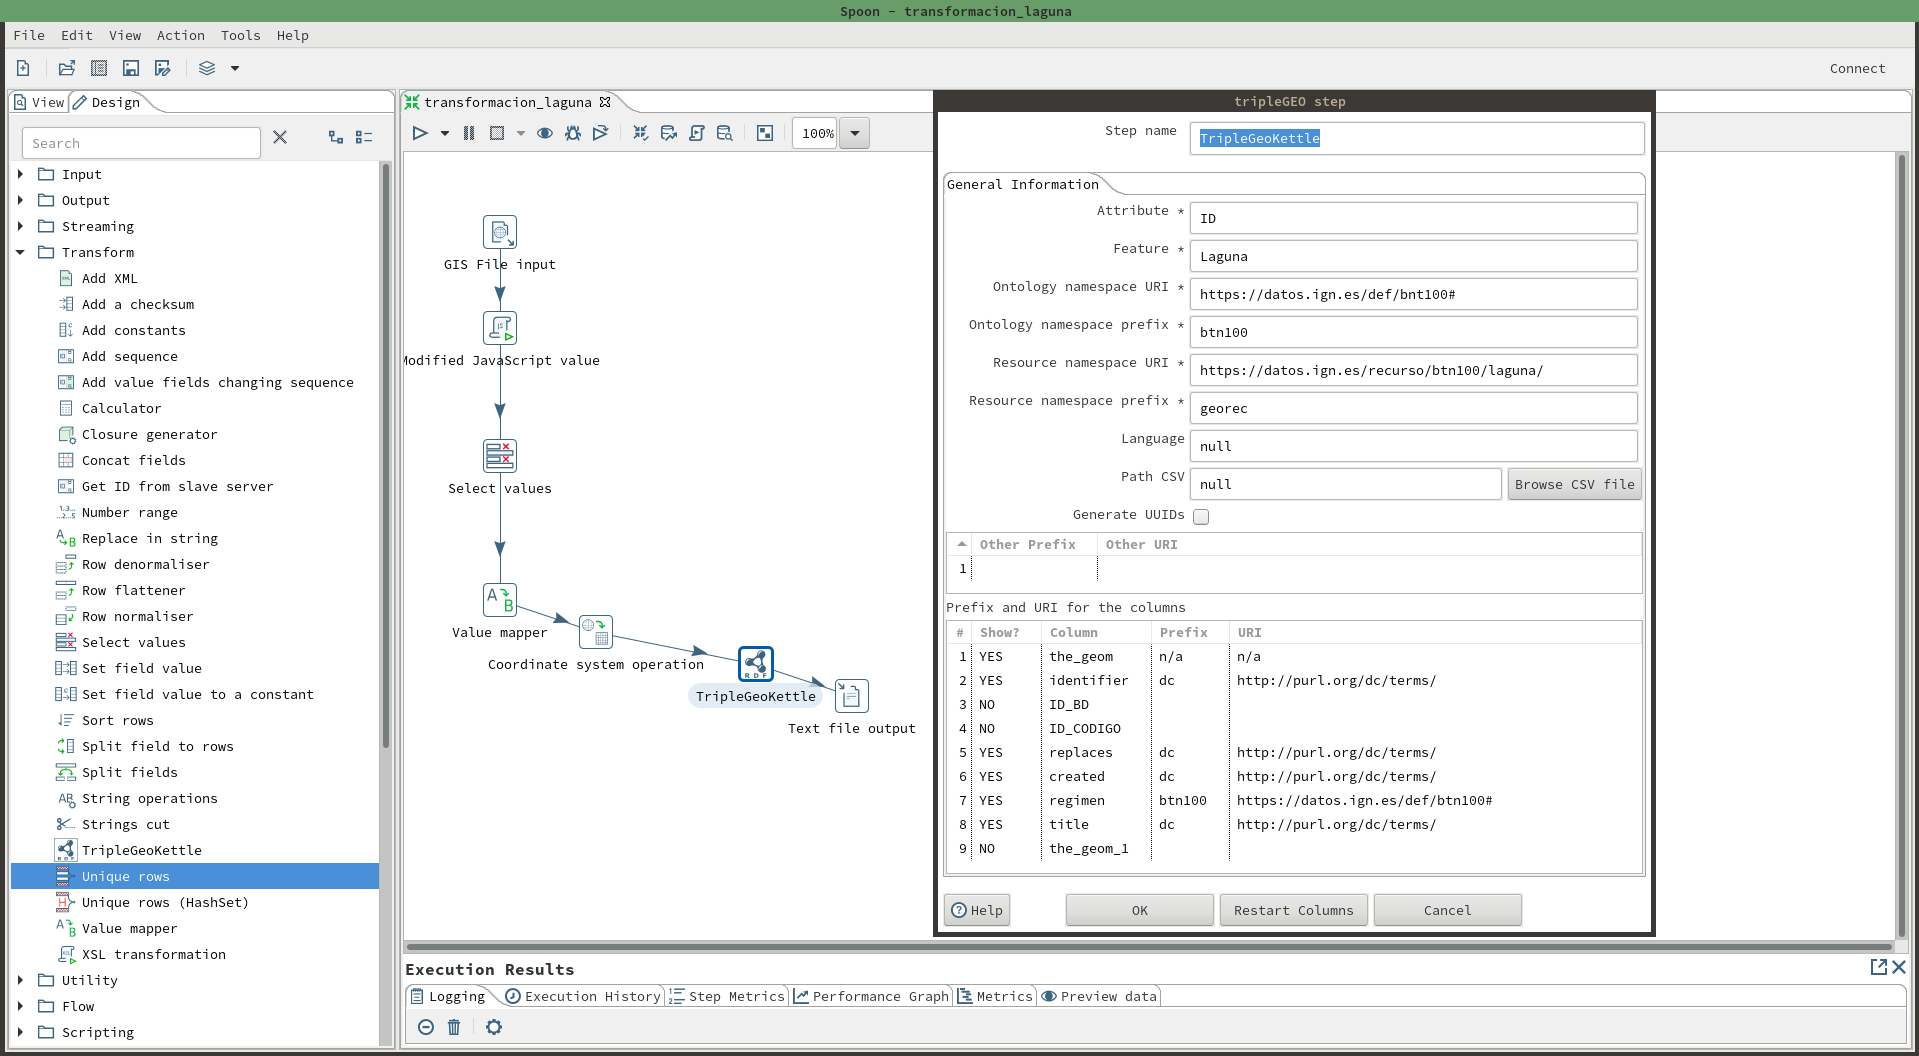
\includegraphics[width=\textwidth]{images/TGK-portado.png}
    \centering
    \caption{TripleGeoKettle corriendo en PDI9}
    \label{fig:TGK-portado}
\end{figure}


\subsection{Debugging}

Para depurar el plugin se ha creado una nueva configuracion de depuracion eclipse en localhost y el puerto 1044
(fig.\ref{fig:debug-configurations}) y se han anyadido los parametros de ejecucion del script de inicio spoon.sh.

\begin{lstlisting}
if [ -z "\$PENTAHO_DI_JAVA_OPTIONS" ]; then
    PENTAHO_DI_JAVA_OPTIONS="-Xms1024m -Xmx2048m -Xdebug -Xnoagent -Djava.compiler=NONE -Xrunjdwp:transport=dt_socket,server=y,suspend=y,address=1044"
fi
\end{lstlisting}

\begin{figure}[H]
    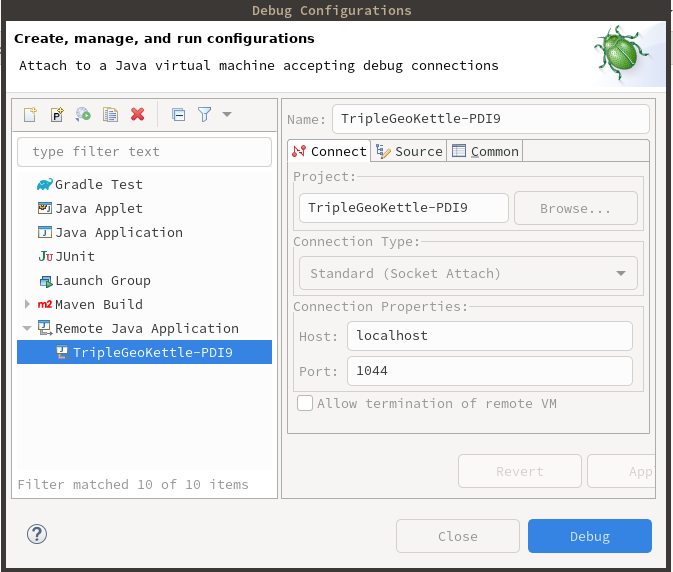
\includegraphics[width=\textwidth]{images/debug-configurations.png}
    \centering
    \caption{Configuracion de depuracion en Eclipse}
    \label{fig:debug-configurations}
\end{figure}

El error NullPointerException se debe a:

\begin{lstlisting}
1. Con la siguiente llamada se inicia el modelo RDF:
    tripleGEOStep.java 160: this.shpToRDF.getModelFromConfiguration();

2. Desde la funcion se crea el modelo con:
    Model modelAux = ModelFactory.createOntologyModel(OntModelSpec.RDFS_MEM);

3. En ese momento salta una exception que no detiene e programa y la variable modelAux se mantiene en null.
    Schema factory class org.apache.xerces.impl.dv.xs.SchemaDVFactoryImpl does not extend from SchemaDVFactory.

4. Despues se utiliza en la funcion
    ShpToRDF.java 176: setModel_rdf(modelAux);

5. Y como modelAux se ha inicializado a null, model_rdf tambien lo es.
    ShpToRDF.java 712: public void setModel_rdf(Model model_rdf) { this.model_rdf = model_rdf; }

6. Finalmente al llamar a la siguiente funcion salta NullPointerException ya que model_rdf es null:
ShpToRDF.java 550:
	private void insertResourceTypeResource(String r1, String r2) {
		this.model_rdf.add(this.model_rdf.createResource(r1), RDF.type, this.model_rdf.createResource(r2));
	}

# Es muy posible que tenga que ver con la version de las librerias de xerces.

# El problema es el siguiente:
Apache Jena y vividsolutions.jts utilizan Xerces, pero versiones distintas. Cuendo funciona uno, el otro falla.

\end{lstlisting}


\subsection{Compilación}

Para el pom.xml de Maven se ha decidido dejar de utilizar maven-assembly-plugin ya que en algunos casos no
incluía los jars necesarios y saltaban errores en tiempo de ejecución. En su lugar se utilizará
maven-shade-plugin que es más apropiado para proyectos grandes con muchas dependencias que pueden tener
conflictos entre sí. Además crea un ``super jar'' que incluye todas las dependencias, tal y como se hacía antiguamente
con el build.xml de Ant.

\begin{lstlisting}
        <build>
        <plugins>
            <plugin>
                <artifactId>maven-compiler-plugin</artifactId>
                <version>3.8.1</version>
                <configuration>
                    <encoding>UTF-8</encoding>
                    <target>${java.version}</target>
                    <source>${java.version}</source>
                </configuration>
            </plugin>
            <plugin>
                <groupId>org.apache.maven.plugins</groupId>
                <artifactId>maven-shade-plugin</artifactId>
                <version>3.2.4</version>
                <executions>
                    <execution>
                        <phase>package</phase>
                        <goals>
                            <goal>shade</goal>
                        </goals>
                    </execution>
                </executions>
            </plugin>
        </plugins>
    </build>
\end{lstlisting}

